\documentclass[12pt]{article}
\usepackage[utf8]{inputenc}
\usepackage{amsmath, amssymb}
\usepackage{xcolor}
\usepackage{geometry}
\usepackage{hyperref}
\usepackage{fancyhdr}
\usepackage{enumitem}
\usepackage{minted}
\usepackage{booktabs}
\usepackage{tikz} 
\usetikzlibrary{positioning}


\geometry{margin=1in}
\hypersetup{colorlinks=true, linkcolor=blue, urlcolor=cyan}

\pagestyle{fancy}
\fancyhf{}
\fancyhead[L]{\textbf{\TOPICTITLE}}
\fancyhead[R]{\thepage}

% -------------------------------
% Topic Metadata
% -------------------------------
\newcommand{\TOPICTITLE}{Application Layer: Web and HTTP}
\title{\TOPICTITLE\\\large Study-Ready Notes}
\author{Compiled by Andrew Photinakis}
\date{\today}

\setlength{\headheight}{15pt}

\begin{document}
\maketitle
\tableofcontents
\newpage

\section*{Keywords}
\noindent\textbf{Keywords:}
\begin{itemize}
    \item Application Layer
    \item Network Applications
    \item Client-Server Paradigm
    \item Peer-to-Peer (P2P) Architecture
    \item Processes and Sockets
    \item Port Numbers
    \item Application-Layer Protocols
    \item HTTP (Hypertext Transfer Protocol)
    \item SMTP (Simple Mail Transfer Protocol)
    \item IMAP (Internet Message Access Protocol)
    \item DNS (Domain Name System)
    \item Transport Layer Services
    \item TCP (Transmission Control Protocol)
    \item UDP (User Datagram Protocol)
    \item Data Integrity
    \item Throughput Requirements
    \item Timing Constraints
    \item TLS (Transport Layer Security)
    \item Socket Programming
    \item CDNs (Content Delivery Networks)
    \item Video Streaming
    \item Network Security
    \item Protocol Design
\end{itemize}



\section{Introduction to Application Layer}
\begin{itemize}
    \item Principles of network applications
    \item Web and HTTP (part 1 and 2)
    \item E-mail, SMTP, IMAP
    \item The Domain Name System: DNS
    \item P2P applications
    \item Video streaming, CDNs
    \item Socket programming with UDP and TCP
\end{itemize}

\textcolor{blue}{[Summary: The application layer is the top layer in network protocols, handling user-facing services like web browsing, email, and file transfer. It defines how applications communicate over networks.]}

\section{Web and HTTP Fundamentals}

\subsection{Web Page Composition}
\begin{itemize}
    \item Web pages consist of multiple \textbf{objects}
    \item Each object can be stored on different web servers
    \item Objects can be: HTML files, JPEG images, Java applets, audio files, etc.
    \item Base HTML file includes references to other objects
    \item Each object is addressable by a \textbf{URL}
\end{itemize}

\textbf{URL Structure:}
\begin{verbatim}
www.someschool.edu/someDept/pic.gif
|              |   |
host name      |   path name
              domain
\end{verbatim}

\subsection{HTTP Overview}
\begin{itemize}
    \item \textbf{HTTP:} Hypertext Transfer Protocol
    \item Web's application-layer protocol
    \item Uses \textbf{client/server model}:
          \begin{itemize}
              \item \textbf{Client:} Browser that requests, receives, and displays web objects
              \item \textbf{Server:} Web server that sends objects in response to requests
          \end{itemize}
\end{itemize}

\begin{figure}[h]
    \centering
    \begin{tabular}{c c c}
        PC running      & $\rightarrow$           & Server running    \\
        Firefox browser & HTTP requests/responses & Apache Web server \\
        iPhone running  & $\rightarrow$           &                   \\
        Safari browser  & HTTP requests/responses &                   \\
    \end{tabular}
    \caption{HTTP Client-Server Architecture}
\end{figure}

\textcolor{blue}{[Summary: HTTP is the foundation of web communication, using a client-server model where browsers request resources and servers provide them.]}

\section{HTTP Connections}

\subsection{Connection Types}
\begin{itemize}
    \item \textbf{Non-persistent HTTP:}
          \begin{enumerate}
              \item TCP connection opened
              \item At most one object sent over TCP connection
              \item TCP connection closed
              \item Downloading multiple objects requires multiple connections
          \end{enumerate}

    \item \textbf{Persistent HTTP:}
          \begin{itemize}
              \item TCP connection opened to a server
              \item Multiple objects can be sent over \textit{single} TCP connection
              \item TCP connection closed after all objects transferred
          \end{itemize}
\end{itemize}

\subsection{Non-persistent HTTP Example}
\textbf{Scenario:} User enters URL: www.someSchool.edu/someDepartment/home.index (contains text + 10 JPEG references)

\begin{enumerate}
    \item HTTP client initiates TCP connection to HTTP server on port 80
    \item HTTP client sends HTTP request message with URL
    \item HTTP server receives request, forms response with requested object
    \item HTTP server closes TCP connection
    \item HTTP client receives response, displays HTML, finds 10 referenced JPEGs
    \item Steps 1-5 repeated for each of 10 JPEG objects
\end{enumerate}

\subsection{Response Time Analysis}
\begin{itemize}
    \item \textbf{RTT (Round Trip Time):} Time for small packet to travel from client to server and back
    \item \textbf{Non-persistent HTTP Response Time:}
          \[ \text{Response Time} = 2 \times \text{RTT} + \text{File Transmission Time} \]
          \begin{itemize}
              \item One RTT to initiate TCP connection
              \item One RTT for HTTP request and first bytes of response
              \item Object/file transmission time
          \end{itemize}
\end{itemize}

\begin{figure}[h]
    \centering
    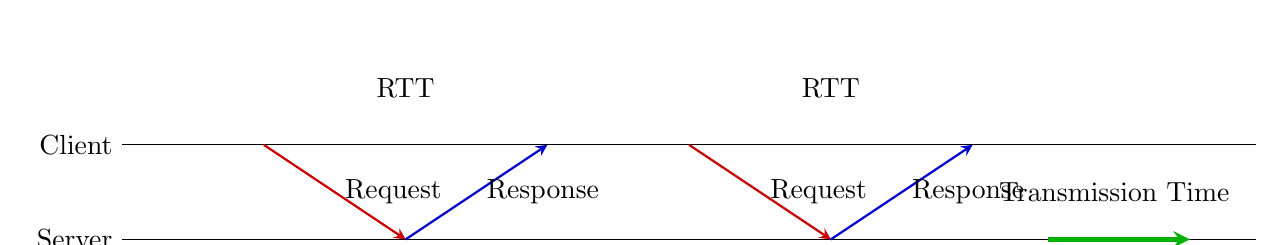
\begin{tikzpicture}[scale=1.2, >=stealth]
        % Client and Server lines
        \draw (0,1) -- (12,1);
        \draw (0,0) -- (12,0);
        \node[left] at (0,1) {Client};
        \node[left] at (0,0) {Server};

        % RTT 1 (Request + Response)
        \draw[->, thick, color=red!80!black] (1.5,1) -- (3,0)
        node[midway, right, black] {Request};
        \draw[->, thick, color=blue!80!black] (3,0) -- (4.5,1)
        node[midway, right, black] {Response};
        \node[above] at (3,1.4) {RTT};

        % RTT 2 (Request + Response)
        \draw[->, thick, color=red!80!black] (6,1) -- (7.5,0)
        node[midway, right, black] {Request};
        \draw[->, thick, color=blue!80!black] (7.5,0) -- (9,1)
        node[midway, right, black] {Response};
        \node[above] at (7.5,1.4) {RTT};

        % Transmission Time
        \draw[->, ultra thick, color=green!70!black] (9.8,0) -- (11.3,0);
        \node[above, black] at (10.5,0.3) {Transmission Time};
    \end{tikzpicture}
    \caption{Non-persistent HTTP Response Time Components (colored by message type)}
    \label{fig:http_rtt}
\end{figure}

\textcolor{orange}{[Mnemonic: Non-persistent = "One and Done" - one object per connection]}
\textcolor{blue}{[Summary: Non-persistent HTTP requires separate connections for each object, leading to 2 RTTs per object, while persistent HTTP reuses connections for multiple objects.]}

\section{Persistent HTTP (HTTP 1.1)}

\subsection{Non-persistent HTTP Issues}
\begin{itemize}
    \item Requires 2 RTTs per object
    \item OS overhead for each TCP connection
    \item Browsers open multiple parallel TCP connections to fetch objects
\end{itemize}

\subsection{Persistent HTTP Advantages}
\begin{itemize}
    \item Server leaves connection open after sending response
    \item Subsequent HTTP messages use same connection
    \item Client sends requests immediately upon encountering referenced objects
    \item As little as one RTT for all referenced objects
    \item Cuts response time in half compared to non-persistent
\end{itemize}

\textcolor{teal}{[Concept Map:
            \begin{itemize}
                \item HTTP 1.0 → Non-persistent → Multiple connections → High overhead
                \item HTTP 1.1 → Persistent → Single connection → Lower overhead
                \item Performance improvement: 2RTT/object → ~1RTT/multiple objects
            \end{itemize}
        ]}

\section{HTTP Message Format}

\subsection{HTTP Request Message}
\begin{itemize}
    \item ASCII (human-readable format)
    \item Two types: request and response messages
\end{itemize}

\textbf{General Format:}
\begin{verbatim}
| method | sp | URL | sp | version | cr | lf |
| header field name | : | value | cr | lf |
| ... |
| cr | lf |
| entity body |
\end{verbatim}

\subsection{HTTP Request Methods}
\begin{itemize}
    \item \textbf{GET:} Request object from server
          \begin{itemize}
              \item Can include user data in URL after '?': www.sombsite.com/animalsearch?monkeys\&banana
          \end{itemize}

    \item \textbf{POST:} Send data to server
          \begin{itemize}
              \item Used for form input
              \item User input sent in entity body
          \end{itemize}

    \item \textbf{HEAD:} Request headers only (no body)
    \item \textbf{PUT:} Upload new file to server
          \begin{itemize}
              \item Completely replaces existing file
          \end{itemize}
\end{itemize}

\subsection{HTTP Response Message}
\begin{itemize}
    \item \textbf{Status line:} protocol + status code + status phrase
    \item Example: HTTP/1.1 200 OK
\end{itemize}

\subsection{HTTP Response Status Codes}
\begin{itemize}
    \item \textbf{200 OK:} Request succeeded, object in message
    \item \textbf{301 Moved Permanently:} Object moved, new location specified
    \item \textbf{400 Bad Request:} Request not understood
    \item \textbf{404 Not Found:} Requested document not found
    \item \textbf{505 HTTP Version Not Supported:} Unsupported protocol version
\end{itemize}

\textcolor{blue}{[Summary: HTTP messages follow specific formats with request methods (GET, POST, HEAD, PUT) and response codes (200, 301, 404, etc.) that indicate request outcomes.]}

\section{HTTP in Practice}

\subsection{Trying HTTP with Netcat}
\begin{enumerate}
    \item Open TCP connection: \texttt{\% nc -c -v gaia.cs.umass.edu 80}
    \item Send GET request:
          \begin{verbatim}
    GET /kurose_ross/interactive/index.php HTTP/1.1
    Host: gaia.cs.umass.edu
    \end{verbatim}
    \item Examine server response
\end{enumerate}

\subsection{HTTP State Management: Cookies}
\begin{itemize}
    \item HTTP is \textbf{stateless} - no memory between requests
    \item \textbf{Cookies} maintain state between transactions
\end{itemize}

\textbf{Four Cookie Components:}
\begin{enumerate}
    \item Cookie header line in HTTP \textit{response} message
    \item Cookie header line in HTTP \textit{request} message
    \item Cookie file on user's host (managed by browser)
    \item Back-end database at website
\end{enumerate}

\begin{figure}[h]
    \centering
    \begin{tabular}{c c c}
        Client       &                  & Server              \\
        Cookie file  & $\rightarrow$    & Backend database    \\
        Amazon: 1678 & HTTP with cookie & ID: 1678, user data \\
    \end{tabular}
    \caption{Cookie-based State Management}
\end{figure}

\begin{figure}[h]
    \centering
    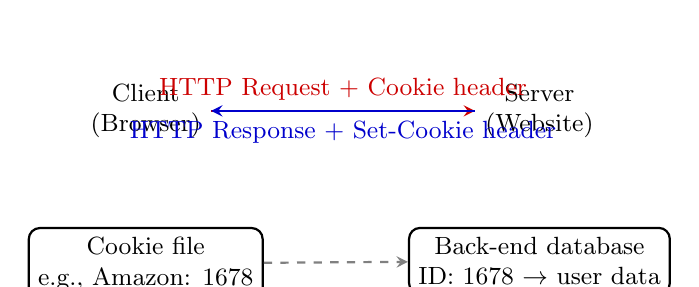
\begin{tikzpicture}[>=stealth, node distance=5cm, thick, font=\small]
        % Nodes
        \node (client) [align=center] {Client \\ (Browser)};
        \node (server) [right of=client, align=center] {Server \\ (Website)};

        % Cookie file and DB
        \node[below=1cm of client] (cookiefile) [draw, rounded corners, align=center] {Cookie file\\ e.g., Amazon: 1678};
        \node[below=1cm of server] (database) [draw, rounded corners, align=center] {Back-end database\\ ID: 1678 $\rightarrow$ user data};

        % Arrows
        \draw[->, color=red!80!black] (client) -- node[above]{HTTP Request + Cookie header} (server);
        \draw[->, color=blue!80!black] (server) -- node[below]{HTTP Response + Set-Cookie header} (client);
        \draw[->, dashed, color=gray] (cookiefile) -- (database);

    \end{tikzpicture}
    \caption{Cookie-based State Management: How client and server maintain user state using cookies.}
    \label{fig:cookie_state}
\end{figure}


\subsection{Cookie Applications and Privacy}
\begin{itemize}
    \item \textbf{Uses:} Authorization, shopping carts, recommendations, user sessions
    \item \textbf{Privacy concerns:}
          \begin{itemize}
              \item Sites learn about user behavior
              \item Third-party persistent cookies track across multiple sites
              \item Common identity tracking
          \end{itemize}
\end{itemize}

\textcolor{orange}{[Mnemonic: Cookies have 4 C's: Client, Cache, Communication, Control]}
\textcolor{blue}{[Summary: Cookies overcome HTTP's stateless nature by storing user-specific data, enabling personalized experiences but raising privacy concerns.]}

\section{Web Caching and Performance}

\subsection{Web Caches (Proxy Servers)}
\begin{itemize}
    \item \textbf{Goal:} Satisfy client requests without origin server involvement
    \item Browser configured to point to local web cache
    \item Cache acts as both client and server
\end{itemize}

\textbf{Cache Operation:}
\begin{enumerate}
    \item Browser sends request to cache
    \item If object in cache: return to client
    \item Else: request from origin server, cache object, return to client
\end{enumerate}

\subsection{Cache Control Headers}
\begin{itemize}
    \item \textbf{Cache-Control: max-age=<seconds>:} Object caching duration
    \item \textbf{Cache-Control: no-cache:} Do not cache object
\end{itemize}

\subsection{Benefits of Web Caching}
\begin{itemize}
    \item Reduce client response time (cache closer to client)
    \item Reduce traffic on institution's access link
    \item Enable efficient content delivery for providers
\end{itemize}

\section{Caching Performance Analysis}

\subsection{Base Scenario}
\begin{itemize}
    \item Access link rate: 1.54 Mbps
    \item RTT to server: 2 seconds
    \item Web object size: 100K bits
    \item Request rate: 15 requests/second
    \item Data rate to browsers: 1.50 Mbps
\end{itemize}

\textbf{Performance without Cache:}
\begin{itemize}
    \item Access link utilization: 0.97 (97\%)
    \item LAN utilization: 0.0015
    \item End-end delay: 2 sec + minutes + microseconds
\end{itemize}
sdf
\subsection{Option 1: Faster Access Link}
\begin{itemize}
    \item Upgrade to 154 Mbps access link
    \item Access link utilization: 0.0097 (0.97\%)
    \item Cost: Expensive
\end{itemize}

\subsection{Option 2: Web Cache}
\begin{itemize}
    \item Install local web cache
    \item Cost: Cheap
\end{itemize}

\textbf{Performance with Cache (40\% hit rate):}
\begin{itemize}
    \item 40\% requests served by cache (low msec delay)
    \item 60\% requests served by origin
    \item Access link data rate: $0.6 \times 1.50 \text{ Mbps} = 0.9 \text{ Mbps}$
    \item Access link utilization: $0.9 / 1.54 = 0.58$
    \item Average end-end delay:
          \[
              \begin{aligned}
                  \text{Delay} & = 0.6 \times (\text{delay from origin}) + 0.4 \times (\text{delay from cache}) \\
                               & = 0.6 \times 2.01 + 0.4 \times (\text{msecs}) \approx 1.2 \text{ seconds}
              \end{aligned}
          \]
\end{itemize}

\textcolor{blue}{[Summary: Web caching dramatically improves performance by serving content locally, reducing both response time and network traffic compared to upgrading infrastructure.]}

\section{Advanced HTTP Features}

\subsection{Conditional GET}
\begin{itemize}
    \item \textbf{Goal:} Avoid sending object if cache has up-to-date version
    \item Client includes: \texttt{If-modified-since: <date>}
    \item Server responses:
          \begin{itemize}
              \item \textbf{304 Not Modified:} Cached copy is current
              \item \textbf{200 OK:} Object modified, new version sent
          \end{itemize}
\end{itemize}

\subsection{HTTP/2}
\begin{itemize}
    \item \textbf{Key goal:} Decrease delay in multi-object requests
    \item Improvements over HTTP 1.1:
          \begin{itemize}
              \item Object transmission based on client-specified priority (not FCFS)
              \item Push unrequested objects to client
              \item Divide objects into frames
              \item Mitigate Head-of-Line (HOL) blocking
          \end{itemize}
\end{itemize}

\subsubsection{HOL Blocking Mitigation}
\begin{itemize}
    \item \textbf{HTTP 1.1:} Objects delivered in request order
          \begin{itemize}
              \item Small objects wait behind large objects
          \end{itemize}
    \item \textbf{HTTP/2:} Objects divided into frames, transmission interleaved
          \begin{itemize}
              \item Small objects delivered quickly
              \item Large objects slightly delayed
          \end{itemize}
\end{itemize}

\subsection{HTTP/3}
\begin{itemize}
    \item \textbf{Limitations of HTTP/2:}
          \begin{itemize}
              \item Single TCP connection means packet loss stalls all objects
              \item Browsers open multiple parallel TCP connections
              \item No security over vanilla TCP
          \end{itemize}
    \item \textbf{HTTP/3 improvements:}
          \begin{itemize}
              \item Adds security
              \item Per-object error and congestion control over UDP
              \item More pipelining capabilities
          \end{itemize}
\end{itemize}

\textcolor{teal}{[Concept Map:
            \begin{itemize}
                \item HTTP 1.0 → Non-persistent → High latency
                \item HTTP 1.1 → Persistent → Reduced connections
                \item HTTP/2 → Frame multiplexing → HOL blocking mitigation
                \item HTTP/3 → UDP-based → Per-object control + security
            \end{itemize}
        ]}

\section*{Exam Questions}

\subsection*{HTTP Fundamentals}
\begin{enumerate}
    \item Compare and contrast persistent vs. non-persistent HTTP connections. What are the performance implications of each?
    \item Calculate the response time for downloading a web page with 5 objects using non-persistent HTTP, given RTT = 100ms and transmission time per object = 50ms.
    \item Explain how cookies overcome HTTP's stateless nature and discuss the privacy concerns associated with them.
\end{enumerate}

\subsection*{Caching and Performance}
\begin{enumerate}
    \item A web cache has a hit rate of 60\%. The average response time for cache hits is 10ms and for cache misses is 200ms. Calculate the overall average response time.
    \item Describe how conditional GET works and why it's beneficial for network performance.
    \item Compare the cost-effectiveness of upgrading access link speed vs. installing a web cache for improving institutional network performance.
\end{enumerate}

\subsection*{HTTP Evolution}
\begin{enumerate}
    \item Explain how HTTP/2 mitigates head-of-line blocking compared to HTTP 1.1.
    \item What are the main advantages of HTTP/3 over HTTP/2, and why was UDP chosen as the transport protocol?
    \item Describe a scenario where HTTP/2's object prioritization would provide significant performance benefits over HTTP 1.1.
\end{enumerate}

\textcolor{red}{[Exam Questions: These questions cover key concepts including HTTP connection types, performance calculations, caching benefits, and protocol evolution from HTTP 1.1 to HTTP/3.]}

\end{document}